

\Chapter{Generation}{RQ1. To what extent it is possible to artificially create resilient variants for WebAssembly programs?} 

% What is this chapter about ?
%Our hypothesis is that we can increase the diversity of software applications through the mean of functionally equivalent transformations. We propose a methodology and the theoretical foundation to achieve this goal.
%In this chapter, we evaluate the feasibility of having a diversifier by using the same strategy a superoptimizers follow.


%\section{}

In this chapter, we investigate whether we can artifically create program variants through semantically equivalent code transformations. We propose a framework to create WebAssembly program variants that are functionally equivalent to their original, yet exhibit a different behavior.
We propose to retarget a superoptimizer, using its exhaustive searching strategy for providing semantically equivalent code transformations that are discarded due to its non-optimal nature.
The presented methodology and transformation tool, CROW, are contributions to this thesis.
We evaluate the usage of CROW on a corpus of open-source and nature diverse programs. 
We sum up the key insights taken from this evaluation.


\section{CROW}
\label{section:crow}
In this section we describe CROW, a tool tailored to create semantically equivalent variants out of a single program, either C/C++ code or LLVM bitcode. CROW is part of the contribution of this thesis.
In \autoref{diagrams:crow}, we describe the workflow of CROW to create program variants.

\begin{figure*}[h]
    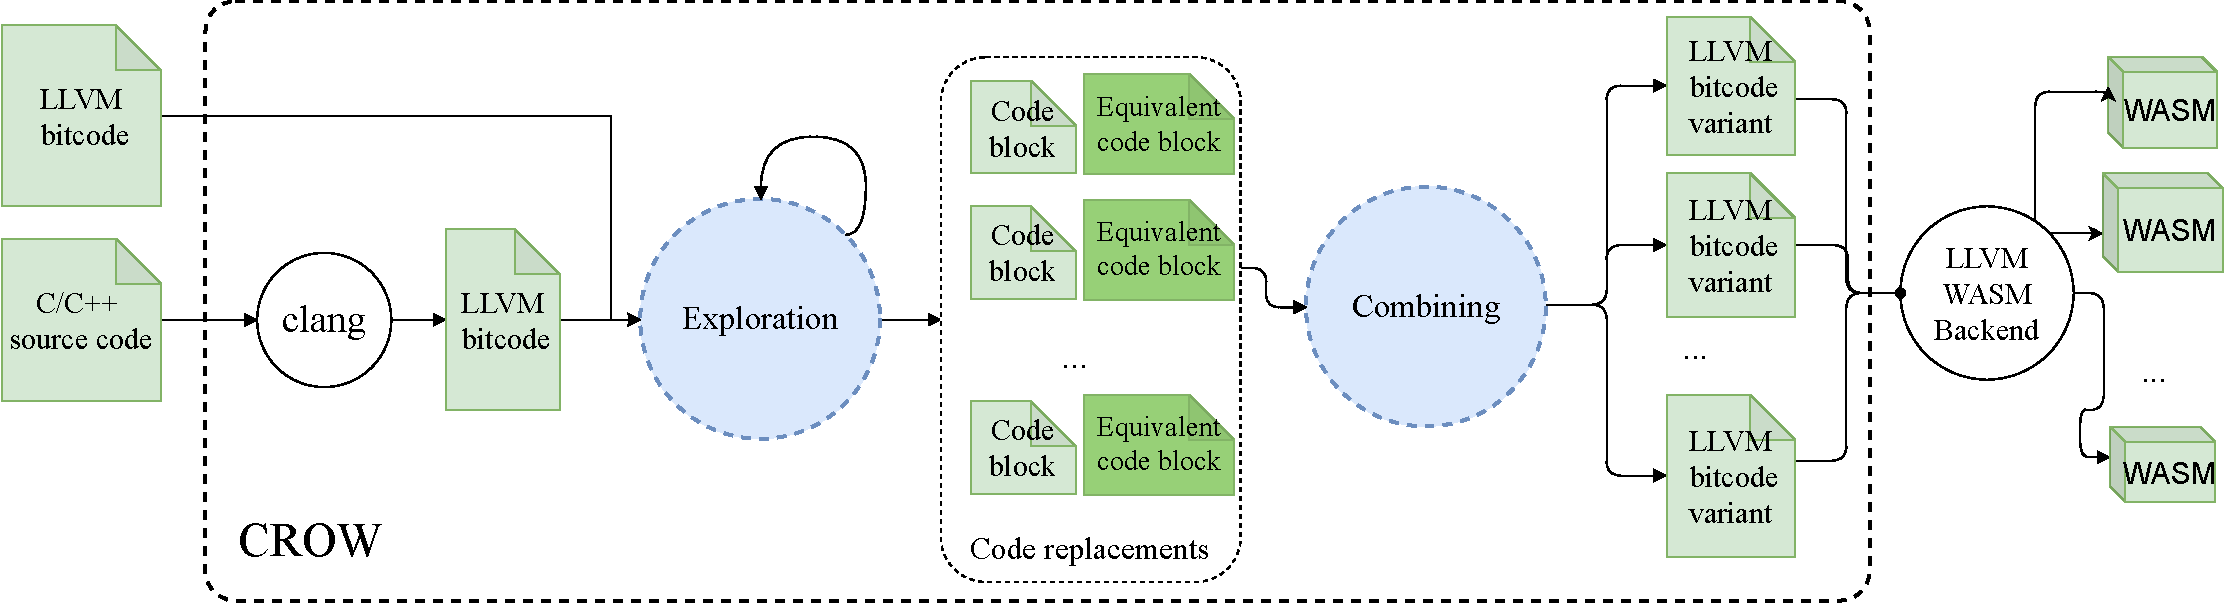
\includegraphics[width=\linewidth]{diagrams/generation/crow.drawio.pdf}
    \caption{TODO}
    \label{diagrams:crow}
\end{figure*}

%This assumption is motivated as follows: first, LLVM-based compilers are the most popular compilers to build \wasm programs \cite{usenixWASM2020}; second, the availability of source code (typically C/C++ for \wasm) provides a structure to perform code analysis and produce code replacements that is richer than the binary code.

CROW synthesizes program variants to be \wasm programs. We assume that the programs are generated through the LLVM compilation pipeline. This assumption is supported by the work of Lehman et al. \cite{} and the fact that Wasm programs are generated in the 60\% of the times by the LLVM toolchain.

During the \emph{exploration} stage, CROW takes as input a C/C++ programs or LLVM bitcodes and produces a set of unique, diversified LLVM bitcodes that can be later ported to \wasm.
Figure \ref{diagrams:crow} shows the stages of this workflow. The workflow starts with compiling the input program into LLVM bitcode using clang if it comes from source code or LLVM bicode. Then, CROW analyzes the bitcode to synthesize a set of candidate code replacements. In the following we enunciate the definitions we use along this work for code block, functional equivalence and code replacement. 


\begin{definition}{Block (based on Aho \etal \cite{10.5555/6448}):}\label{def:code-block}
    Let $P$ be a program. A block $B$ is a grouping of declarations and statements in $P$ inside a function $F$. 
\end{definition}


\begin{definition}{Functional equivalence modulo program state (based on Le \etal \cite{10.1145/2594291.2594334}):}
    \label{def:functional-equivalence}
    Let $B_1$ and $B_2$ be two code blocks according to \autoref{def:code-block}. We consider the program state before the execution of the block, $S_i$, as the input and the program state after the execution of the block, $S_o$, as the output. $B_1$ and $B_2$ are functionally equivalent if given the same input $S_i$ both codes produce the same output $S_o$.
\end{definition}

\begin{definition}{Code replacement:}
    \label{def:code-replacement}
    Let $P$ be a program and $T$ a pair of code blocks $(B_1, B_2)$. $T$ is a candidate code replacement if $B_1$ and $B_2$ are both functionally equivalent as defined in \autoref{def:functional-equivalence}.
    Applying $T$ to $P$ means replacing $B_1$ by $B_2$. The application of $T$ to $P$ produces a program variant $P'$ which consequently is functionally equivalent to $P$.     
\end{definition}

We address the \emph{exploration} stage  by retargeting a  superoptimizer for  LLVM, Souper, using its subset of the LLVM intermediate representation. CROW uses it at function level, taking the functions inside the LLVM bitcode module as individual instances to analyze and diversify/ The retargeted superoptimizer is in charge of finding the potential places in the original code functions where a replacement can be applied. Also, it makes the formal verification of \autoref{def:functional-equivalence} using a theorem prover. 
On the other hand, we prevent the superoptimizer from synthesizing instructions that have no correspondence in \wasm for sake of reducing the searching space for equivalent program variants.

\todo{We disable cost restrictions and the LLVM backend optimizations...maybe for the assesment RQ ?}

Finally, In the \emph{combining} stage, CROW combines the candidate code replacements to generate different LLVM bitcode variants. In this stage, we select and combine code replacements that have been synthesized during the exploration stage. We apply each code replacement to the original program to produce a LLVM IR variant.
Then, this IR is compiled into a \wasm binary if requested. CROW generates the variants from all possible combinations of code replacements as the power set over all code replacements. \todo{Add motivation about why we need to generate the power set. } 

\subsection{Example}
\label{section:crow:example}
 Let us illustrate how CROW works with the simple example code in \autoref{CExample}. The \texttt{f} function calculates the value of $2 * x + x$ where \texttt{x} is the input for the function.  This code is compiled by CROW generating the intermediate LLVM bitcode in the left most part of \autoref{example:crow:original:llvm}. As the right-most part of \autoref{example:crow:original:llvm}, CROW potentially found two variants for the variable $\%2$ in line X.  

 \begin{code}
    \lstset{language=C,caption={C function that calculates the quantity $2x + x$},label=CExample}
    \begin{lstlisting}[style=CStyle]
    int f(int x) { 
        return 2 * x + x; 
    }
    
    int main(void) { return f(10); }
    \end{lstlisting}
    
    \end{code}

 \lstdefinelanguage{LLVM}
    {morekeywords={i32,mul,align,nsw,add,load,store,define,br, ret, shl, ret},
    sensitive=false,
    morecomment=[l]{;},
    morecomment=[s]{;}{;},
    morestring=[b]",
}
\lstdefinestyle{nccode}{
    numbers=left,
    tabsize=4,
    showspaces=false,
    breaklines=true, 
    showstringspaces=false,
    moredelim=**[is][{\btHL[fill=black!10]}]{`}{`},
    moredelim=**[is][{\btHL[fill=celadon!40]}]{!}{!}
}
\lstset{
    language=LLVM,
    style=nccode,
    %basicstyle=\small\ttfamily,
    columns=fullflexible,
    breaklines=true
}

\todo{Add arrows from the candidates to the original code.}

\begin{code}
    \centering
    \captionof{lstlisting}{LLVM's intermediate representation program and code transformations.}\label{example:crow:original:llvm}
    \lstset{numbers=none}
    \noindent\begin{minipage}[b]{.55\linewidth}
    \centering
    \begin{lstlisting}[xleftmargin=1em]
    define i32 @f(i32) {
     %2 = mul nsw i32 %0,2 %*\label{line:original:first:start}*)
     %3 = add nsw i32 %0,%2 %*\label{line:original:second:start}*)
     
     ret i32 %3
    }
    
    define i32 @main() {
     %1 = tail call i32 @f(i32 10)
     ret i32 %1
    }
    \end{lstlisting}
    \end{minipage}\hfill%
    \noindent\begin{minipage}[b]{.4\linewidth}
    \vspace{-10pt}
        \lstdefinestyle{nccode}{
          tabsize=4, 
          showspaces=false,
          breaklines=true, 
          showstringspaces=false,
        moredelim=**[is][{\btHL[fill=black!10]}]{`}{`},
        moredelim=**[is][{\btHL[fill=celadon!40]}]{!}{!}
        }
        \lstset{
            language=LLVM,
            style=nccode,
            columns=fullflexible,
            breaklines=true,
            belowcaptionskip=1pt,
            abovecaptionskip=1pt,
        }
        \vfill%
        \begin{lstlisting}[label={ref:block1} ,name={A}]
    %2 = mul nsw i32 %0,2
        \end{lstlisting}
        \begin{lstlisting}[name={B}]
    %2 = mul nsw i32 %0,2
    %3 = add nsw i32 %0,%2
        \end{lstlisting}
    \end{minipage}
\end{code}

\todo{Add all the found examples here}

CROW, in the exploration stage, can synthesize $6 + 1$ bitcode variants, which results in $14$ module variants (the power set combination size). Yet, the generation stage would eventually generate $7$ variants from the original \wasm binary. This gap between the number of potential and the actual number of variants is a consequence of the redundancy among the bitcode variants when composing several variants into one. 

\section{Evaluation}
\label{section:crow:exp_setup}

We use CROW and method described at \autoref{section:crow} to answer RQ1. In this section we describe the corpora of original programs that we pass to CROW for sake of variants generation. Besides, we describe our metrics, and we finalize by discussing the results.

\subsection{Corpora}
\label{section:crow:corpora}

We answer RQ1 with two corpora of programs appropriate for our experiments. The first corpus, \textbf{CROW prime}, is part of the CROW contribution \cite{}. The second corpus, \textbf{MEWE prime}, is part of the MEWE contribution \cite{}. In \autoref{table:corpora} we summarize the selection criteria, and we sum up the properties of each corpus. With both corpora we evaluate CROW wih a total of $303 + 7$ programs, containing $303 + 1902$ functions.

\begin{table}[H]
    \renewcommand{\arraystretch}{1.8}
    \footnotesize
    \centering
    \begin{tabular}{p{1cm} p{6cm} p{5cm}}
        Corpus name & Selection criteria & Corpus Description \\
        \midrule
        \textbf{CROW prime} & To build the corpus used in CROW, we take programs from the  Rosetta Code project\footnote{\url{http://www.rosettacode.org/wiki/Rosetta_Code}}. 
        %This website hosts a curated set of solutions for specific programming tasks in various  programming languages.
        %It contains a wide range of tasks, from simple ones, such as adding two numbers, to complex algorithms like a compiler lexer. 
        We first collect all C programs from Rosetta Code, which represents $989$ programs as of 01/26/2020. 
        
        We then apply a number of filters: the programs should successfully compile, they should not require user inputs, the programs should terminate and should not provide in non-deterministic results.  
        The result of the filtering is a corpus of 303 C programs  &  All programs have a single function in terms of source code. These programs range from $7$ to $150$ lines of code and solve a variety of problems, from the \textit{Babbage} problem to  \textit{Convex Hull} calculation. \\
        \hline
        \textbf{MEWE prime} & We select two mature and typical edge-cloud computing projects for this corpus.
        The projects are selected based on: suitability for  diversity synthesis with CROW (the projects should have the ability to collect their modules in LLVM intermediate representation)
        
        %, suitability for deployment on the Fastly infrastructure (the project should be easily portable Wasm/WASI and compatible with the Rust Fastly API). 

        The selected projects are: \textbf{libsodium}, an encryption, decryption, signature and password hashing library which can be ported to WebAssembly and \textbf{qrcode-rust}, a QrCode and MicroQrCode generator written in Rust. We then filter out 5 and 2 endpoints\footnote{We consider and endpoint as a public available function in the compiled project, \ie functions that can be easily called without a complicated harnss.} respectively, for which we select their involved functions. 
        
        &  The evaluated projects contains in total 1902 functions, $62$ for libdosium and $1840$ for qrcode-rust. The function range between 10 ad 127700 lines of code. \\
    \end{tabular}
    \caption{Corpora description. The table is composed by the name of the corpus, the selection criteria and the stats the programs in each corpus.}
    \label{table:corpora}
\end{table}



\subsection{Setup and evaluation}

CROW's workflow synthesizes program variants with an enumerative strategy. This means that all possible programs that can be generated for a given language (LLVM in the case) are constructed and verified for equivalence.
There are two parameters to control the size of the search space and hence the time required to traverse it.
On one hand, one can limit the size of the variants. On the other hand, one can limit the set of instructions that are used for the synthesis. In our experiments, we use between $1$ instruction (only additions) and $60$ instructions (all supported instructions in the synthesizer).


These two  configuration parameters allow the user to find a trade-off between the amount of variants that are synthesized and the time taken to produce them. In \autoref{table:corpora:setup} we listed the configuration for both corpora. For the current evaluation, given the size of the corpus, we set the exploration time to 1 hour maximum per function for \textbf{CROW PRIME}, for a total of 303 hours CROW executions. In the case of \textbf{MEWE prime} we set the timeout to 6 minutes per function in the exploration stage. We set all 60 supported instructions in CROW for both \textbf{CROW prime} and \textbf{MEWE primer} corpora.

\begin{table}[h]
    \renewcommand{\arraystretch}{1.2}
    \centering
    \begin{tabular}{l l l}
        \midrule
        CORPUS & Timeout & Max. instructions \\
        \hline
        CROW prime & 1h & 60 \\
        \hline
        MEWE prime & 6m & 20 \\
    \end{tabular}
    \caption{CROW tweaking for variants generation. The table is composed by the name of the corpus, the timeout parameter and the maximum number of instructions allowed per variant.}
    \label{table:corpora:setup}
\end{table}


With RQ1,
we assess the ability of our approach to generate \wasm binaries that are statically different from the original program.
For this, we compute the number of unique variants generated by CROW for each original program. 
We compare the \wasm program and its variant using the \texttt{md5} hash as a metric. 

% Move this to the next chapter, assesment
%Since \wasm binaries are further transformed into machine code before they execute, we also check that this additional transformation preserves the difference introduces by CROW in the \wasm binary. We use the Turbofan ahead-of-time compiler of V8, with all its possible optimizations, to generate a x86 binary for each \wasm binary. Then, we compare the x86 version of each variant against the x86 binary corresponding to the original \wasm binary.

% Replace DTW here by the sha comparison


%Dynamic Time Warping (DTW)  \cite{Maia08usinga}. DTW computes the global alignment between two sequences. It returns a value capturing the cost of this alignment, which is actually a distance metric, called DTW. The larger the DTW distance, the more different the two sequences are. In our case, we compare the sequence of instructions of each variant with the initial program and the other variants. We obtain two DTW distance values for each program-variant pair: one at the level of \wasm code and the another one at the level of x86 code. \autoref{metric:static1} below defines these metrics.


%\begin{metric}{Md5:}
%    \label{metric:static1}
%    Given a program $P$, its \texttt{md5} hash is the result of encoding its bytestream using the md5 algorithm.
%\end{metric}


\section{Results}

We summarize the results in \autoref{table:crow:general_results}
CROW produces at least one unique program variant for $239/303{}$ programs for \textbf{CROW prime} with 1h for timeout. For the rest of the programs ($64/303{}$), the timeout is reached before CROW can find any valid variant. 
In the case of \textbf{MEWE prime}, CROW produces equivalent variants for $48/1902$ original programs with 6 minutes per function as timeout. The rest of the programs resulted timeout before finding function variants or produced none.

{
    \renewcommand{\arraystretch}{1.6}
\begin{table}[h]
    \centering
    %\setlength\minrowclearance{1.0pt}
        \begin{tabular}[t]{ l  l  l  l  l }
            \midrule
        CORPUS & \#Functions & \# Diversified & \# NonDiversified & \# Variants  \\
        \hline   

        CROW prime & 303 & \textbf{239} & 64 & 1906    \\
        \hline
        MEWE prime & \pypy{\allmewefunctions} & \pypy{\allmewediversified} & \pypy{{\allmewefunctions} - {\allmewediversified}} & \textbf{\pypy{\allmewepopulation}}    \\
        \hline


        \end{tabular}
    
        \caption{General diversification results. The table is composed by the name of the corpus, the number of functions, the number of succesfully diversified functions, the number of non-diversified functions and the cumulative number of variants.}
        \label{table:crow:general_results}
\end{table}
}

\todo{Expand this}

\subsection{Properties for large diversification using CROW}

We made a manual analysis of the programs that yield more than 100 unique variants to study the key properties of programs leveraging a high number of variants.
This reveals one key reason that favors many unique variants: the programs include  bounded loops. In these cases CROW
synthesizes variants for the loops by unrolling them. Every time a loop is unrolled, the loop body is copied and moved as part of the outer scope of the loop. This creates a new, statically different, program. The number of programs grows exponentially with nested loops. 

A second key factor for the synthesis of many variants relates to the presence of arithmetic. Souper, the synthesis engine used by CROW, is effective in replacing  arithmetic instructions by equivalent instructions that lead to the same result. For example, CROW generates unique variants by replacing multiplications with additions or shift left instructions (\autoref{add:example}). Also, logical comparisons are replaced, inverting the operation and the operands (\autoref{cmp:examples}). On the other hand, CROW is able to use the instrinsics of the computation model to create equivalent variants using overflow and underflow of integers to produce variants (\autoref{overflow:example}).


\begin{code}
    \scriptsize
    \lstdefinestyle{nccode}{
        numbers=none,
        firstnumber=2,
        stepnumber=1,
        numbersep=10pt,
        tabsize=4, 
        showspaces=false,
        breaklines=true, 
        showstringspaces=false,
        moredelim=**[is][\btHL]{`}{`},
        moredelim=**[is][{\btHL[fill=black!10]}]{`}{`},
        moredelim=**[is][{\btHL[fill=celadon!40]}]{!}{!}
    }

    \lstset{
        language=WAT,
        style=nccode,
        basicstyle=\footnotesize\ttfamily,
        columns=fullflexible,
        breaklines=true
    }
    \noindent\begin{minipage}[b]{0.32\linewidth}
        \captionof{lstlisting}{Diversification through arithmetic expression replacement.}\label{add:example}
        \noindent\begin{minipage}[t]{0.46\linewidth}
            \begin{lstlisting}
local.get 0
`i32.const 2`
`i32.mul`
            \end{lstlisting}
        \end{minipage}%
        \hfill\noindent\begin{minipage}[t]{0.46\linewidth}
            
            \begin{lstlisting}
local.get 0
!i32.const 1!
!i32.shl!
            \end{lstlisting}
        \end{minipage}
    \end{minipage}\hfill%
    \begin{minipage}[b]{0.31\linewidth}
        \captionof{lstlisting}{Diversification through inversion of comparison operations.}\label{cmp:examples}
        \begin{minipage}[t]{.46\linewidth}
            \begin{lstlisting}
`local.get 0`
`i32.const 10`
`i32.gt_s`
            \end{lstlisting}
        \end{minipage}\hfill\begin{minipage}[t]{.46\linewidth}
           
            \begin{lstlisting}
!i32.const 11!
!local.get 0!
!i32.le_s!
            \end{lstlisting}
        \end{minipage}%
        
        
    \end{minipage}\hfill\noindent
    \noindent\begin{minipage}[b]{0.32\linewidth}
        \captionof{lstlisting}{Diversification through overflow of integer operands.}\label{overflow:example}
        \noindent\begin{minipage}[t]{0.46\linewidth}
            \begin{lstlisting}
`TODO`
            \end{lstlisting}
        \end{minipage}%
        \hfill\noindent\begin{minipage}[t]{0.46\linewidth}
            
            \begin{lstlisting}
!TODO!
            \end{lstlisting}
        \end{minipage}
    \end{minipage}
    \end{code}


% \input{parts/example_rq1_replacements}



% \input{parts/example_rq1_babbage}


%We now discuss the prevalence of the transformations made by CROW when the \wasm binaries are transformed to machine code, specifically with the V8's engine. In \autoref{fig:rq1} we plot the cumulative distribution of
%\DTWStatic{}, comparing \wasm binaries (in blue) and x86 binaries (in orange). The figure plots  a total of 103003 \DTWStatic{} values for each representation, two values for each variant pair comparison (including original) for the 239 program.
%The value on the y-axis shows which percentage of the total comparisons lie below the corresponding \DTWStatic{} value on the x-axis.
%Since we measure the distances between original programs and \wasm variants, then $100\%$ of these  binaries have $\DTWStatic{}>0$.
%Let us consider the x86 variants: \DTWStatic{} is strictly positive for \nPreservedPercent{} of variants. In all these cases, the V8 compilation phase does not undo the CROW diversification transformations.
%Also, we see that there is a gap between both distributions, the main reason is the natural inflation of machine code. For example, two variants that differ by one single instruction in \wasm, can be translated to machine code where the difference is increased by more than one machine code instruction.

% Negative prevalence
%The zoomed subplot focuses on the beginning of the distribution, it shows that the \DTWStatic{} is zero for $0.52\%$ of the x86 binaries.
%In these cases the V8 TurboFan compiler from \wasm to x86 reverts the CROW transformations.
%We find that CROW produces at least one of these reversible transformations for $34/303Diversified{}$ programs.
%\autoref{add:prevalence_example} shows one of the most common transformations that is reversed by TurboFan, according to our experiments.

%Besides, local variables reordering and common subexpressions are cases that TurboFan reverses.
%\input{parts/non-prevalence-example}



\subsection{Challenges for automatic diversification}

CROW generates variants for functions in both corpora, however, we have observed a remarkable difference between the number of successfully diversified functions versus the number of failed-to-diversify functions, as it can be appreciated in \autoref{table:crow:general_results}. CROW succesfully diversified approx. 79\% and 2.5\% of the original functions for \textbf{CROW prime} and  \textbf{MEWE prime} respectively. On the other hand, CROW generated more variants for \textbf{MEWE prime}, 4670 program variants for 48 original programs. Not surprisingly, to set the timeout affects the capacity of CROW for diversification. On the other hand, a low timeout for exploration \todo{Define above that the timeout is for exploration} gives CROW more power of combining code replacements, generating more variants. This can be appreciated in the last column of the table, where for a lower number of diversified functions CROW created, overall, more variants.


Moreover, we look at the cases that yield a small number of variants per function. There is no direct correlation between the number of identified code for replacement and the number of unique variants. We manually analyze programs that include a significant number of potential places for replacements, for which CROW generates few variants. 
We identify three main challenges for diversification.

\emph{1) Constant computation}  We have observed that Souper searches for a constant replacement for more than $45\%$ of the blocks of each program while constant values cannot be inferred. For instance,  constant values cannot be inferred for memory load operations because CROW is oblivious to a memory model. 

\todo{Add example here}

% candidates overlapping
\emph{2) Combination computation}  The overlap between code blocks, discussed in \autoref{section:crow:example}, is a second factor that limits the number of unique variants. CROW can generate a high number of variants, but not all replacement combinations are necessarily unique.

\todo{Add example here}


\subsection{Variants properties}

Regarding the potential size overhead of the generated variants, we have compared the \wasm binary size of the 239 programs with their variants. The ratio of size change between the original program and the variants ranges from 82\% (variants are smaller) to 125\% (variants are larger) for \textbf{CROW prime}. This limited impact on the binary size of the variants is good news because they are meant to save bandwidth when they become assets to distribute over network.


\section{Conclusions}

\todo{}